\subsection{Pattern Matching DTW}

\newcommand{\dtw}{\mathrm{DTW}}
\newcommand{\ed}{\mathrm{ED}}
\newcommand{\RLE}{\mathrm{RLE}}


\begin{frame}
    \centering
    {\Large Pattern Matching Under Dynamic Time Warping Distance}
  
    \bigskip
    {\large SPIRE'22}\\
    \bigskip
    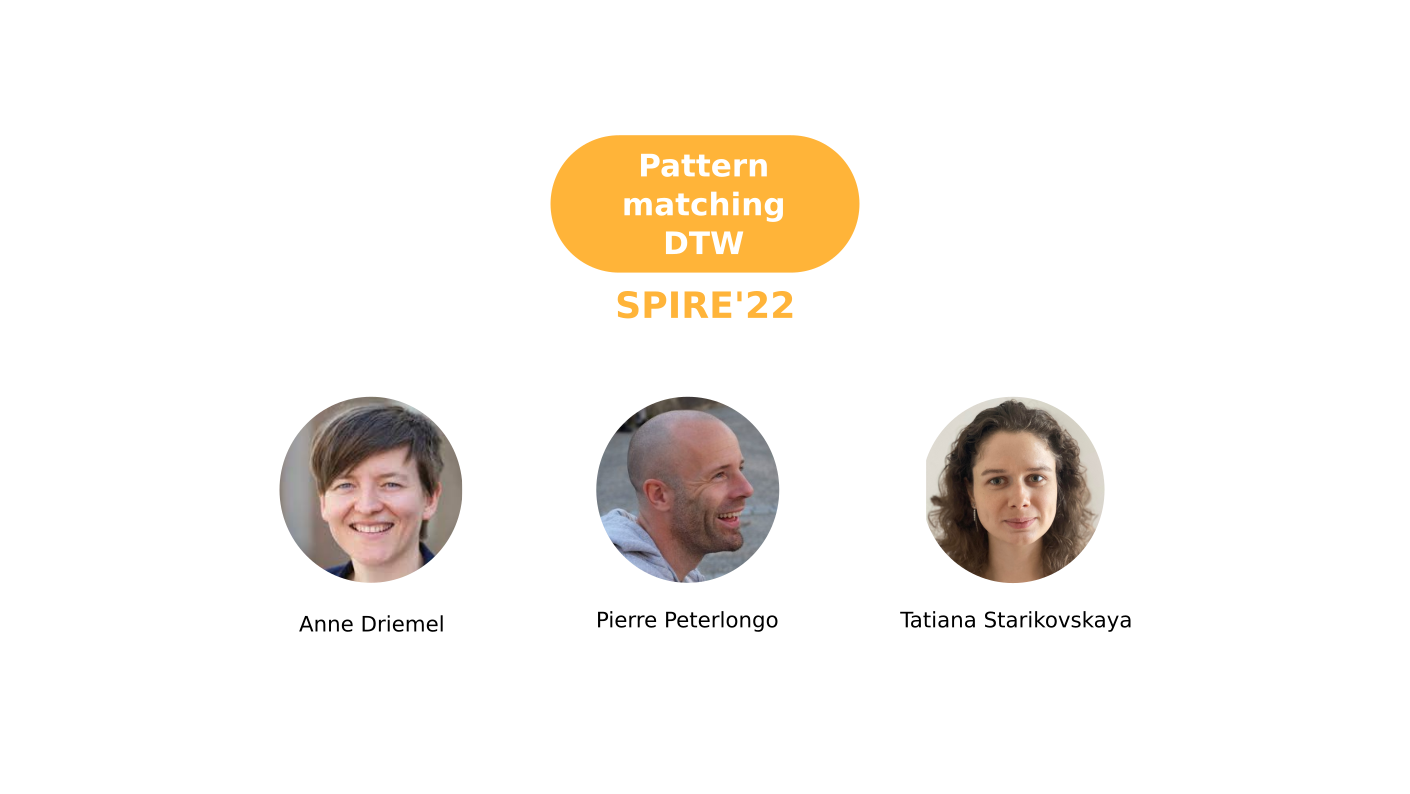
\includegraphics{pictures/mindmap/dtw.png}
  
    \bigskip
    Anne Driemel, Pierre Peterlongo, Tatiana Starikovskaya
\end{frame}


\begin{frame}{Dynamic time warping (DTW) distance: comparing time series}

\btheme{Definition:} Minimal distance obtained by \ntheme{duplicating} some items (maintaining equal length) and then \ntheme{summing the distances} between items at the same position.

\begin{center}
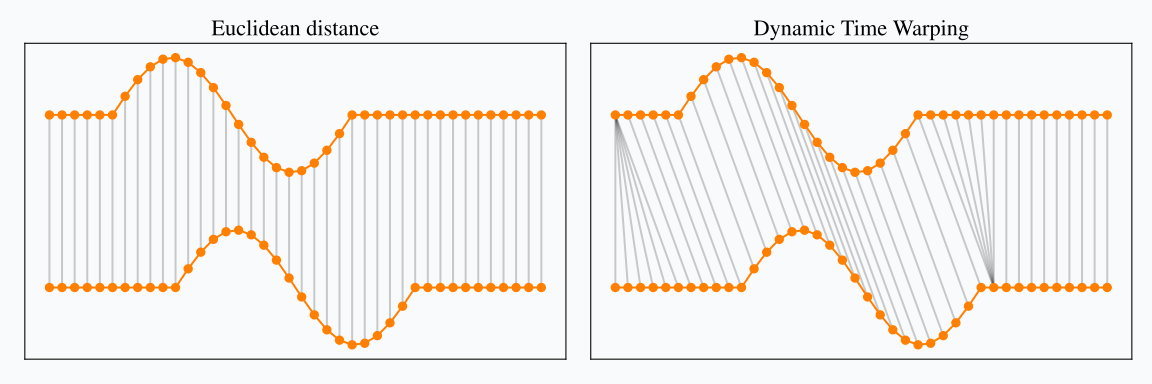
\includegraphics[scale=0.3]{figures/dtw_vs_euc.png}\\
\tiny{Figure credit: Romain Tavenard}
\end{center}
\pause
\small
Used in \ntheme{speech recognition} to deal with varying speeds and more generally for parametrized curves where each item is a \ntheme{multidimensional point}.\pause

\vfill
But what about \btheme{strings}, where the items are characters from a finite alphabet $\Sigma$ ?
\end{frame}

\begin{frame}{Dynamic time warping (DTW) distance for strings}

\begin{columns}
\column{0.5\textwidth}
Given $X$ and $Y$ strings, $\dtw(X,Y)$ is the
minimal distance obtained by \ntheme{duplicating} some characters (maintaining equal length) and then \ntheme{summing the distances} between characters at the same position.
\vfill
\column{0.4\textwidth}

\onslide<2->{
\begin{mdframed}
\center
{\tiny Distance between characters = Hamming distance.} 
\footnotesize
\begin{figure}
%\missingfigure{Under construction...}
\centering
\begin{tikzpicture}[scale=0.6, every node/.style={scale=0.8}]
\foreach \x[count=\i] in {C,A,A,A,G,G} {
    \node at ($(\i, 1)$) {\small{\x}};
}
\foreach \y[count=\j] in {A,T,G} {
    \node at ($(0.5+\j*1.5, 0)$) {\small{\y}};
}
% align A
\fill[mygreen!25] (2, 0.25) -- (2,0.75) -- (4,0.75) -- (2.1,0.25) -- cycle;
% align G
\fill[mygreen!25] (5, 0.25) -- (5,0.75) -- (6,0.75) -- (5.1,0.25) -- cycle;
%draw misalignment
\draw[dashed,red] (1.75, 0.25) -- (1,0.75);
\draw[dashed,red] (3.5, 0.25) -- (5,0.75);
\end{tikzpicture}
\end{figure}
\vfill 
$\dtw($CAAAG$,$ATG$)=2$\\
\end{mdframed}}

\end{columns}
\pause


\onslide<3->{

\btheme{Dynamic Programming}\\
\smallskip
$D$ a matrix of size $(|X|+1)(|Y|+1)$ such that $D[i,j]=\dtw(X[1..i],Y[1..j])$\pause
\bigskip

\btheme{Initialization}~~~$D[0,0]= 0$ and for all $(i,j)$, $D[0,j]=D[i,0]=+\infty$.\\
\bigskip
\btheme{Recurrence} ~~~ 
    $D[i,j] = \min\{$\beamermathcolor{black}
        $\underbrace{\mathcolor{black!30!blue}{D[i-1,j-1]}}_\text{align},
        \underbrace{\mathcolor{black!30!blue}{D[i-1,j]}}_\text{dupl. from Y},
        \underbrace{\mathcolor{black!30!blue}{D[i,j-1]}}_\text{dupl. from X}$
    $\mathcolor{black!30!blue}{\}+ d(X[i], Y[j])}$.
}

\end{frame}


\begin{frame}{Why is DTW on strings interesting? Third generation sequencing}
    \small
    When DNA is sequenced, we obtain fragments (reads) of the DNA that have to be assembled.\pause
    \begin{columns}
    \column{0.4\textwidth}
    \smallskip
    \btheme{Third generation sequencing}\\
    \smallskip
    \textcolor{mygreen}{Long reads, fast and portable.}\\
    \smallskip
    \textcolor{red}{Higher error rate.}\\
    \smallskip
    Uneven speed of the DNA through the nanopore, creates errors on the length when the same nucleotide is repeated (homopolymers/runs)...
    \column{0.5\textwidth}
    \begin{center}
    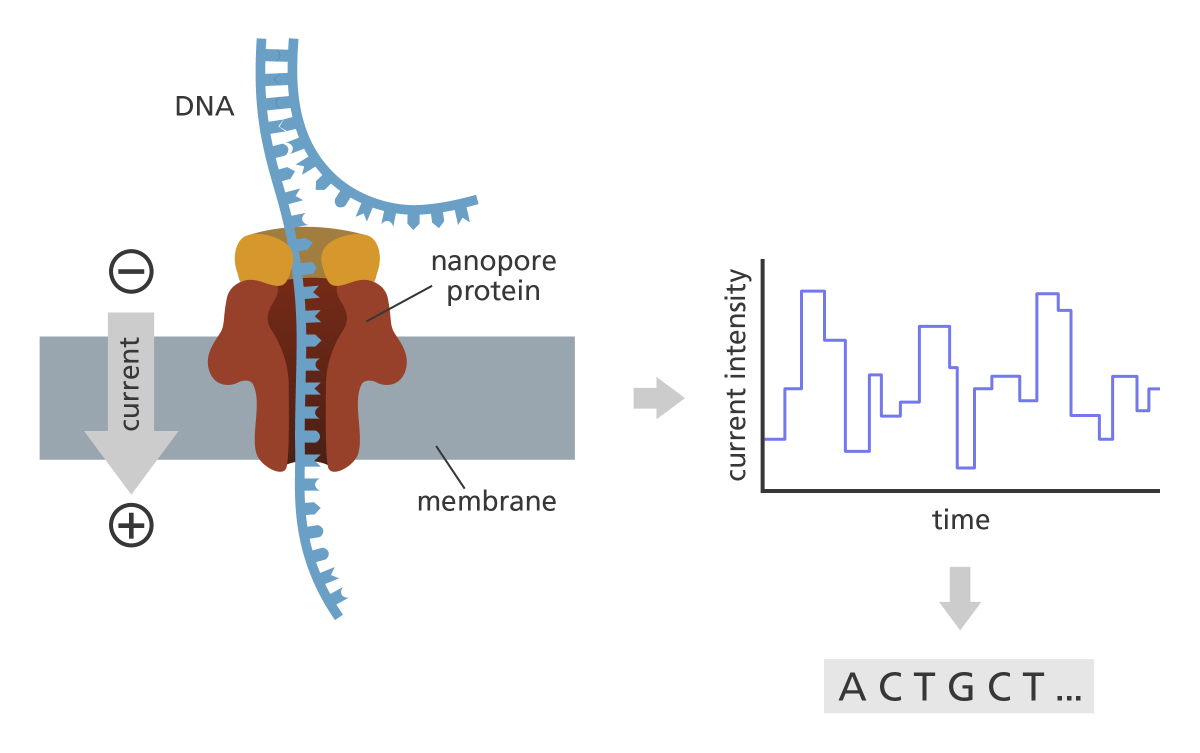
\includegraphics[scale=0.20]{figures/ont-sequencing_yourgenome.png}\\
    {\tiny Figure credit: \href{https://www.yourgenome.org/facts/what-is-oxford-nanopore-technology-ont-sequencing/}{yourgenome.org}}
    \end{center}
    
    \end{columns}\pause
    \vfill
    { DTW  was already used to \ntheme{align the raw signal} by [Loose et al. 2016] and [Han et al. 2020].\\ \pause
    We propose to use it to \ntheme{align the reads (strings)} to a reference (string).\\ \pause
    So we want to find the position where it aligns best ($\neq$ similarity btw. two strings)?}
    
\end{frame}

\begin{frame}{Our subject: pattern matching for DTW}

    \begin{columns}
    \column{0.45\textwidth}
    \begin{mydefblock}{Pattern matching DTW}
        \btheme{Input}~~two strings $P$ and $T$.\\ 
        \btheme{Output}~~for every $0 \leq j < |T|$, 
        ~~~$\min_{0 \leq i \leq j} \dtw(P,T[i..j])$.
    \end{mydefblock}
    
    \column{0.4\textwidth}
    \vfill
    \btheme{Dynamic Programming}\\
    \smallskip
    \ntheme{Changes the Initialization}\\
    for all $0\leq j\leq |T|$, $D[0,j]= 0$ and 
    for all $1 \leq i \leq |P|$, $D[i,0]=+\infty$.\\
    \vfill
    \end{columns}
    \pause
    
    \smallskip
    \noindent\textcolor{gray}{\rule{\textwidth}{0.1pt}}

    \smallskip
    \btheme{State of the art} to compute $\dtw(X,Y)$  with $N=|X|$ and $M=|Y|$:\pause
    
    \medskip
    The dynamic programming takes $\Oh(NM)$. \pause Conditional lowerbound by \ntheme{[Gold and Sharir]} indicates that \textcolor{red}{strongly subquadratic algorithms are unlikely}.\pause

    \medskip
    What if $X$ and $Y$ are made of consecutive repetitions of the same character ``runs'', $n$ and $m$ runs respectively? \pause
    $\Oh(mN+Mn)$-time \ntheme{[Froese et al. Algorithmica'22]} \pause

    To compute the distance only if $\dtw(X,Y) < k$, \pause $\Oh(kN)$-time is possible \ntheme{[Kuszmaul ICALP'19]}. \pause

    \medskip
    \textcolor{red}{Can we also use (and combine) those approaches for Pattern Matching?}
\end{frame}


\begin{frame}{Runs simplify the dynamic programming matrix}
    $T$ and $P$ strings, $N=|T|$ and $M=|P|$, with $n$ and $m$ runs. \pause
    \smallskip

    If $P[i_p.. j_p]$ is a run in $P$, and $T[i_t .. j_t]$ is a run in $T$.\pause
    
    
    %
\begin{center}
\footnotesize
\resizebox{0.8\textwidth}{!}{
\begin{tabular}{|cc||cc|cccc|c|cc|c|cccc|cc|c|c|c|c|c|}
\hline
 &   & G & G & T & T & T & T & C & T & T & A & T & T & T & T & G & G & T & G & A & T & A \\
 & 0 & 0 & 0 & 0 & {0} & 0 & 0 & 0 & 0 & 0 & 0 & 0 & 0 & 0 & 0 & 0 & 0 & 0 & 0 & 0 & 0 & 0 \\
\hline
A  & $\infty$  & 1 & 1 & \textcolor{red}{1} & \textcolor{red}{1} & \textcolor{red}{1} & \textcolor{red}{1} & 1 & 1 & 1 &{ 0 } & 1 & 1 & 1 & 1 & 1 & 1 & 1 & 1 &{ 0 } & 1 &{ 0 }\\
A  & $\infty$  & 2 & 2 & \textcolor{red}{2} & \textcolor{red}{2} & \textcolor{red}{2} & \textcolor{red}{2} & 2 & 2 & 2 &{ 0 } & 1 & 2 & 2 & 2 & 2 & 2 & 2 & 2 &{ 0 } & 1 &{ 0 }\\
\hline
T  & $\infty$  & 3 & 3 &{ 2 } &{ 2 } &{ 2 } &{ 2 } & {3} &{{ 2 }} &{{ 2 }} & 1 &{ 0 } &{ 0 } &{ 0 } &{ 0 } & 1 & 2 &{ 2 } & 3 & 1 &{ 0 } & 1\\
T  & $\infty$  & 4 & 4 &{ 2 } &{ 2 } &{ 2 } &{ 2 } & 3 & {{ 2 }} &{{ 2 }} & 2 &{ 0 } &{ 0 } &{ 0 } &{ 0 } & 1 & 2 &{ 2 } & 3 & 2 &{ 0 } & 1\\
\hline
A  & $\infty$  & 5 & 5 & 3 & 3 & 3 & 3 & 3 & 3 & {3} &{{ 2 }} & 1 & 1 & 1 & 1 & 1 & 2 & 3 & 3 &{ 2 } & 1 &{ 0 }\\
\hline
T  & $\infty$  & 6 & 6 &{ 3 } &{ 3 } &{ 3 } &{ 3 } & 4 &{ 3 } &{ 3 } &{3} &{{ 1 }} &{{ 1 }} &{{ 1 }} &{{ 1 }} & 2 & 2 &{ 2 } & 3 & 3 &{ 1 } & 1\\
\hline

\end{tabular} }
\end{center}




    {\beamermathcolor{black}
    \[
        D[i,j] = {\min\{D[i-1,j-1],D[i-1,j],D[i,j-1]\}
        + \underbrace{d(T[i], P[j])}_\text{\textcolor{red}{Constant!}}}
    \]
    }

    \pause       
    We call $D[i_p .. j_p, i_t .. j_t]$ a \btheme{\emph{block}}, and there the values are \ntheme{non-decreasing along a row/column/diagonal}. \pause
    We take the shortest path inside a block $\rightarrow$ $\Oh(Nm+Mn)$ time.\\ \pause
    If $d$ is an integer distance, the values $\leq k$ can take \ntheme{at most $k$ distinct values}... \pause
    
    \begin{myalertblock}{Driemel, Gourdel, Peterlongo, Starikovskaya - SPIRE'22}
        For an \textcolor{red}{integer} distance $d: \Sigma \times \Sigma \rightarrow \mathbb{Z}^+$, given $P$ and $T$ run-length compressed with $m$ and $n$ runs resp.,
        we can compute all $\dtw$ distances $\leq k$ in $\Oh(k mn)$ time.
    \end{myalertblock}
    \end{frame}

\begin{frame}{Summary - Pattern Matching for DTW}
    \textbf{Similarity measure:} the Dynamic Time Warping distance on string can be used to align reads with homopolymers errors onto a reference genome.

    \vfill
    
    \textbf{Sketch as input:} Run-length compression sketch, suited to the metric, that allows a complexity proportional to the size of the sketch not the original input.
    
    \vfill
    \begin{myalertblock}{Driemel, Gourdel, Peterlongo, Starikovskaya - SPIRE'22}
        For an \textcolor{red}{integer} distance $d: \Sigma \times \Sigma \rightarrow \mathbb{Z}^+$, given $P$ and $T$ run-length compressed with $m$ and $n$ runs resp.,
        we can compute all $\dtw$ distances $\leq k$ in $\Oh(k mn)$ time.
    \end{myalertblock}
    \vfill
    \textbf{Not shown about this work:} $\Oh(n+m)$ algorithm for $k=1$, \ntheme{approximations} results, and \ntheme{experiments}.


    \smallskip
    \textbf{Open questions:} faster algorithms? \textcolor{gray}{\beamermathcolor{gray} $\tilde{\Oh}(nm)$ [Boneh et al. arxiv'23]}\\ Is $\tilde{\Oh}(k(n+m))$ space and time possible?
\end{frame}
    